%%%%%%%%%%%%%%%%%%%%%%%%%%%%%%%%%%%%%%%%%%%%%%%%%%%%%%%%%%%%%%%%%%%%%%%%%%%%%%%%
%%%                               80 COLONNES                                %%%
%%%%%%%%%%%%%%%%%%%%%%%%%%%%%%%%%%%%%%%%%%%%%%%%%%%%%%%%%%%%%%%%%%%%%%%%%%%%%%%%

\chapter{Évaluation et comparaison des implantations
         de deux protocoles MAC~/ RDC~: ContikiMAC et S-CoSenS}
\chaptermark{Protocoles MAC~/ RDC}
\label{ChProtocolesMAC}

Avant de détailler nos recherches et travaux sur les protocoles MAC~/
RDC, nous allons brièvement détailler le matériel que nous avons
utilisé lors de nos premiers travaux.

%%%%%%%%%%%%%%%%%%%%%%%%%%%%%%%%%%%%%%%%%%%%%%%%%%%%%%%%%%%%%%%%%%%%%%%%%%%%%

\section{Premières plates-formes matérielles}
\label{SecHWMSP430}

Nous avons employé, pour le début de ces travaux de thèse, des \lang{motes}
basées sur des microcontrôleurs d'architecture MSP430. Cette architecture,
conçue par Texas Instruments, offre une consommation d'énergie très basse,
un prix réduit, et de bonnes performances, grâce à une conception RISC
16 bits spécifique. Elle est très couramment utilisée dans les \lang{motes}
utilisées dans les réseaux de capteurs sans-fil. Elle est également
supportée par le simulateur Cooja \cite{Cooja} (par le biais de l'émulateur
MSPSim \cite{MSPSim} intégré à ce dernier), ce qui permet d'effectuer des
simulations permettant de concevoir et de tester facilement des scénarios
de réseaux sans-fil, notamment lorsque de nombreux noeuds sont impliqués.

\bigskip

Les matériels que nous avons utilisés dans un premier temps sont~:

\begin{description}

\item [La TelosB] \cite{DSTelosB}--- également appelée \nom{SkyMote} selon
le constructeur d'origine.\\
Ce matériel a en effet la spécificité d'être une architecture libre, conçue
par l'université de Berkeley, et est donc produite par plusieurs fabricants
différents (Crossbow~/ Memsic, Sentilla, AdvanticSys, etc.).
\newpage
Cet appareil est conçu autour~:
\begin{itemize}
\item du microcontrôleur TI MSP430F1611 \cite{DSMSP430F1611} cadencé à 8~MHz,
comportant 48~Ko de mémoire Flash (programme) et 10~Ko de RAM (données),
\item de l'émetteur~/ récepteur radio TI ChipCon CC2420 \cite{DSCC2420},
\item d'un port USB pour la communication notamment avec un PC,
\item de divers capteurs intégrés (lumière, et humidité~/ température
en option),
\item d'une mémoire Flash externe au microcontrôleur (1~Mo),
\item et d'une antenne intégrée (utilisation possible d'une antenne externe
en option).
\end{itemize}
Cette \lang{mote} est maintenant de conception ancienne, et plusieurs
appareils concurrents sont apparus sur le même segment de marché.

\item [La Zolertia Z1] \cite{DSZ1}--- est l'un de ces concurrents. Son
constructeur, Zolertia~/ Advancare, l'a conçu comme une évolution plus
puissante et (relativement) compatible de la TelosB. Il ne s'agit pas
comme la TelosB d'un \lang{design} matériel libre, Zolertia~/ Advancare
est donc l'unique source de ce matériel.\\
Cet appareil est conçu autour~:
\begin{itemize}
\item du microcontrôleur TI MSP430F2617 \cite{DSMSP430F2617} cadencé à 16~MHz,
comportant 92~Ko de mémoire Flash (programme) et 8~Ko de RAM (données),
\item de l'émetteur~/ récepteur radio TI ChipCon CC2420 \cite{DSCC2420}
\item d'un port micro-USB pour la communication notamment avec un PC,
\item de divers capteurs (accéléromètre 3D et température),
\item de bus d'extension permettant la connexion de capteurs
supplémentaires (<<~Phidgets~>>)
\item d'une mémoire Flash externe au microcontrôleur (2~Mo),
\item et d'une antenne intégrée (utilisation possible d'une antenne externe
en option).
\end{itemize}
Ce matériel, bien que plus récent, est assez répandu, et utilisé
industriellement (notamment sous Contiki).\\
Une version destinée au déboguage (notamment avec un adaptateur JTAG
intégré) est disponible auprès de Zolertia~/ Advancare~: Z1 Starter
Platform \cite{DSZ1SP}.

\end{description}

Notons qu'outre l'architecture des microcontrôleurs, ces deux matériels
présentent de nombreuses similitudes~: une consommation énergétique très
faible (les deux appareils sont conçus pour être alimentés par des piles
AAA classiques), la même puce radio (émettant sur la bande 2,4~GHz
à 250~Kbps), et des performances de même ordre (bien que sensiblement
supérieures pour la Z1).

Les deux appareils utilisent également un cristal d'une fréquence de
32768~Hz (cristal de montre à quartz) comme base de temps pour leurs
\lang{timers}, ce qui a toute son importance pour des utilisations en
temps-réel comme nous le verrons plus bas.

%%%%%%%%%%%%%%%%%%%%%%%%%%%%%%%%%%%%%%%%%%%%%%%%%%%%%%%%%%%%%%%%%%%%%%%%%%%%%

%% Note : le doublement de \sectionmark{} est nécessaire
%%        au bon fonctionnement de cette commande ;
%%        la présence de la version "courte optionnelle"
%%        dans \section est également obligatoire
\section[Implantation de S-CoSenS sous RIOT OS~: précision de la \\
         synchronisation entre noeuds]
        {Implantation de S-CoSenS sous RIOT OS~:
         précision de la synchronisation entre noeuds%
         \sectionmark{Implantation de S-CoSenS sous RIOT OS}}
\sectionmark{Implantation de S-CoSenS sous RIOT OS}
\label{SecSCoSensRIOTPrecSync}

Comme nous l'expliquons en fin de section \vref{PtEchecSCosensContiki},
nous n'avons pas réussi à implanter de façon satisfaisante le protocole
S-CoSenS sous Contiki OS, à cause des limitations imposées par ce dernier.
Nous avons alors fait le choix de RIOT OS comme plate-forme logicielle
pour l'ensemble de nos travaux de thèse.

Une fois notre plate-forme logicielle de travail choisie, puis améliorée et
déboguée notamment grâce nos contributions (détaillées en section
\vref{SecRIOTContrib}), notre premier objectif a été de valider notre
implantation de S-CoSenS sous RIOT, puis nous avons ensuite cherché
à la comparer avec l'implantation standard de ContikiMAC sous Contiki OS.

Pour ces expérimentations, nous avons principalement utilisé, pour des
raisons pratiques, le simulateur Cooja plutôt que des tests sur du matériel
réel. Tous les noeuds simulés lors de nos expérimentations sont des
Zolertia Z1.

Nous avons néanmoins effectué quelques tests de vérification sur du matériel
(voir section \vref{SubsecExpMat}) malheureusement légèrement différent de
nos noeuds simulés, aucun matériel identique n'étant disponible (les
noeuds matériellement les plus proches des Zolertia Z1 nous étant
accessibles en quantité sur un \lang{testbed} étant les WSN430 d'IoT-LAB,
qui sont similaires aux TelosB~/ SkyMotes).

Nous avons ainsi programmé des applications de test sur ces \lang{motes}
virtuelles, et exécuté des simulations sur un PAN (\lang{``Personal
Area Network''}) constitué d'un noeud central dit <<~routeur~>>
et de dix <<~noeuds-feuilles~>> (ou noeuds simples, ou noeuds terminaux).
Ces dix noeuds simples envoient régulièrement des trames de données au
routeur, qui les retransmet lui-même vers un concentrateur (\lang{``sink''})
situé à proximité. La topologie de ce PAN virtuel est représentée figure
\vref{FigVirtualPAN1}.

Dans ce PAN virtuel~:
\begin{itemize}
\item les dix noeuds-feuilles sont tous à la portée les uns des autres,
\emph{et} à la portée du routeur~;
\item le \lang{``sink''} est à la portée du routeur, mais d'aucun autre
noeud~;
\item le routeur est à le seul noeud portée de tous les autres,
sans exception.
\end{itemize}
Cette configuration a été volontairement mise en place pour assurer
un trajet en deux étapes (\lang{``two-hop transmission''}) pour les trames
entre les noeuds-feuilles de départ et la destination (le \lang{``sink''}).

\begin{figure}[!hbt]
\centering
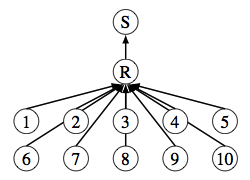
\includegraphics[width=5.5cm]{images/ch5-virtual-pan-test-1.png}
\flcaption{Schéma fonctionnel de notre PAN virtuel de test.\\
(Légende~: \textbf{R}~= noeud routeur~; \textbf{S}~= ``sink'')}
\label{FigVirtualPAN1}
\end{figure}


\newcommand{\nodeid}[1]{\textsf{#1}}


Nos premiers tests ont fait fonctionner le routeur et les dix noeuds simples
exclusivement sous le protocole S-CoSenS \cite{KR-SENSORNETS-2015}. Le but
de ces premiers essais était de vérifier la précision de la synchronisation
entre les différents appareils composant le PAN.

Cooja simule ici un médium radio <<~idéal~>>, sans bruit, affaiblissement
ou autres problèmes survenant en réel. Tous les noeuds sont à la portée
les uns des autres, sans zone d'ombre.

Ces tests ont clairement montré une excellente synchronisation entre les
noeuds-feuilles et le routeur, grâce à la granularité temporelle très fine
du système de gestion des évènements de RIOT OS (et plus particulièrement
la possibilité d'utiliser directement les différents \lang{timers} matériels
disponibles). Cette synchronisation peut être observée sur la copie d'écran
de notre simulation Cooja, visible en figure \vref{FigEcranCooja1}
\footnotemark[1].
Pour une meilleure lisibilité, la portion centrale de la fenêtre
\lang{``timeline''} (délimitée par un rectangle jaune épais) a été zoomée
en figure \vref{FigZoomTimelineCooja1}

\footnotetext[1]{\textbf{Note~:} bien que le titre de la figure
\vref{FigEcranCooja1} mentionne Contiki (dont le projet est à l'origine
du simulateur Cooja), les applications simulées fonctionnent bel et bien
sous RIOT OS.}


\begin{figure}[!p]
\raggedright
\begin{sideways}
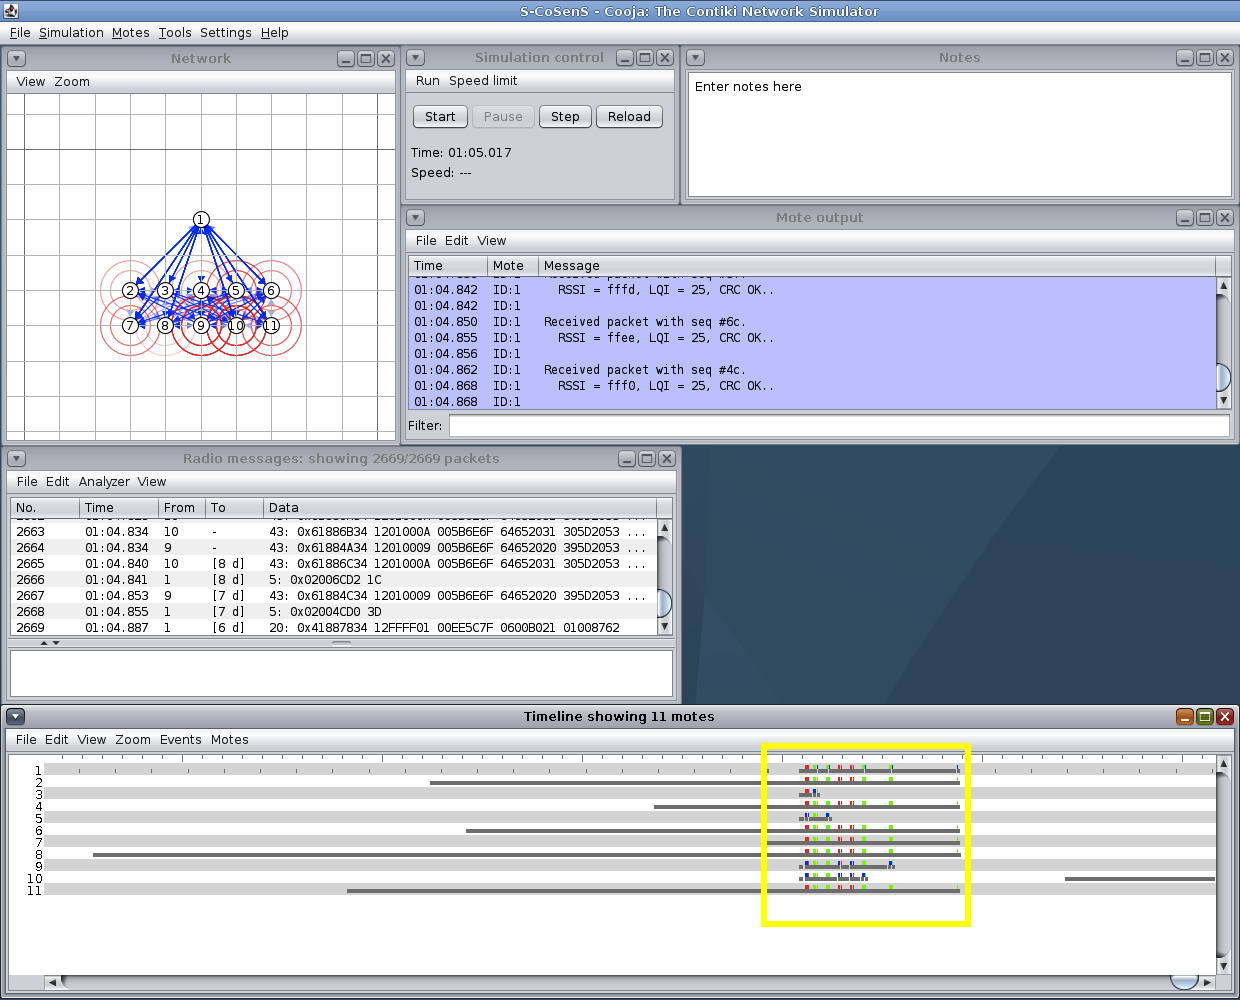
\includegraphics[width=17.4cm]{images/ch5-s-cosens-cooja-1.png}
\end{sideways}
\flcaption{Copie d'écran d'une des simulations de notre premier jeu de
tests sous Cooja.}
\label{FigEcranCooja1}
\end{figure}


\begin{figure}[pbt]
\centering
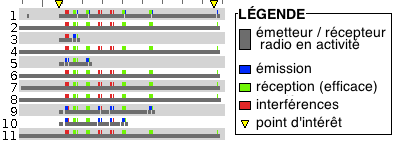
\includegraphics{images/ch5-s-cosens-timeline-1.png}
\flcaption{Zoom sur la partie centrale de la \lang{timeline} de la
figure \vref{FigEcranCooja1}.}
\label{FigZoomTimelineCooja1}
\end{figure}


Sur la figure \vref{FigZoomTimelineCooja1}, les nombres situés à gauche
représentent les identifiants numériques (ID) des \lang{motes}~: le routeur
possède l'ID numéro \nodeid{1}, tandis que les noeuds-feuilles ont les IDs
\nodeid{2} à \nodeid{11}. Les barres grises représentent les périodes
d'activité (écoute active ou transmission) de l'émetteur~/ récepteur radio
d'une \lang{mote} donnée. Les barres bleues représentent l'émission d'une
trame, et les barres vertes la réception \emph{réussie} d'une trame,
tandis que les barres rouges représentent des collisions (quand plusieurs
appareils émettent simultanément) et correspondent ainsi à la présence
sur le canal radio de signaux indéchiffrables.

La figure \vref{FigZoomTimelineCooja1} représente un court instant
(environ 100~millisecondes), correspondant à la fin d'un cycle radio du
routeur~: les 20 premières millisecondes correspondent à la fin de la
période  de sommeil SP (voir le mode de fonctionnnement de S-CoSenS en
section \vref{ParSCoSenS}), et les 80~millisecondes suivantes
représentent la période d'écoute WP, avant le début d'un nouveau cycle
radio (la période de retransmission TP du routeur ayant été désactivée
dans la simulation montrée sur ces copies d'écran pour une meilleure
lisibilité).

Dans l'exemple de la figure \vref{FigZoomTimelineCooja1}, quatre noeuds
ont des données à transmettre au routeur~: les \lang{motes} numéro \nodeid{3},
\nodeid{5}, \nodeid{9} et \nodeid{10}~; les autres noeuds (\nodeid{2},
\nodeid{4}, \nodeid{6}, \nodeid{7}, \nodeid{8} et \nodeid{11}) se préparent
eux à transmettre une trame durant le cycle suivant.

À l'instant marqué par la première flèche jaune (en haut à gauche de la
figure \vref{FigZoomTimelineCooja1}), la période de sommeil SP se
termine et le routeur active son émetteur~/ récepteur radio pour entrer
en période d'écoute WP. On notera que les quatre noeuds ayant des trames
à émettre (\nodeid{3}, \nodeid{5}, \nodeid{9} et \nodeid{10}) activent
également leur radio \emph{précisément} au même instant (à un \lang{tick}
de \lang{timer} soit environ 30 microsecondes près)~: ceci grâce à la
précision des mécanismes temps-réel de RIOT OS (basé sur les \lang{timers}
matériels), permettant aux différents noeuds de se synchroniser précisément
sur les valeurs temporelles transmises par le routeur dans le précédent
\lang{beacon} de début de cycle. Grâce à ce même mécanisme, les noeuds
sont capables de passer leur émetteur~/ récepteur radio \emph{et} leur
microcontrôleur en mode basse consommation aux moments adéquats,
le noyau de RIOT OS étant piloté par les interruptions.

Durant la période d'écoute, nous voyons également que plusieurs collisions
se produisent~; celles-ci sont résolues par la méthode CSMA/CA (sur laquelle
est basé S-CoSenS), laquelle oblige les \lang{motes} à attendre un délai
aléatoire avant de réémettre une trame en cas de conflit. Dans cet exemple,
nos quatre noeuds-feuilles peuvent finalement transmettre leur trame au
routeur dans cet ordre~: \nodeid{3} (après une première collision),
\nodeid{5} et \nodeid{10} (après deux autres collisions), et finalement
\nodeid{9}.

Notons que chaque fois que le routeur (ID numéro \nodeid{1}) reçoit une
trame avec succès, un acquittement (ACK) est renvoyé à l'émetteur~: cela
correspond aux barres bleues très fines suivant chaque barre verte sur
la ligne numéro \nodeid{1}.

Finalement, à l'instant marqué par la seconde flèche jaune (en haut à droite
de la figure \vref{FigZoomTimelineCooja1}), la période d'écoute WP
s'achève, et un nouveau cycle commence. En conséquence, le routeur émet un
\lang{beacon} contenant les durées calculées pour les différentes
périodes constituant le nouveau cycle, et qui serviront à la synchronisation
des dix noeuds-feuilles avec le routeur.

Il est à noter que les \lang{beacon}, contrairement aux trames
de données, ne font pas l'objet d'une transmission classique avec un ou
plusieurs destinataire(s) désigné(s) (\lang{``unicast''} ou
\lang{``multicast''}), mais sont émis pour réception par tous les noeuds
à portée d'écoute~: on dit que les \lang{beacons} font l'objet d'une
diffusion (\lang{``broadcast''}). Par conséquent, contrairement aux trames
de données, les \lang{beacons}~--- étant diffusés~--- ne font pas l'objet
d'un acquittement après réception.

Nous pouvons voir que tous les six noeuds attendant de transmettre une
trame durant ce nouveau cycle (\nodeid{2}, \nodeid{4}, \nodeid{6},
\nodeid{7}, \nodeid{8} et \nodeid{11}) se mettent en sommeil (leur
radio et leur microcontrôleur passent en mode basse consommation) juste
après avoir reçu le \lang{beacon}~; comme nous le voyons dans la figure
\vref{FigZoomTimelineCooja1}, ils vont profiter de la précision des
fonctionnalités temps réel de RIOT pour se réveiller précisément quand
le routeur passera en période d'écoute WP et sera ainsi prêt à recevoir
leurs trames.

%%%%%%%%%%%%%%%%%%%%%%%%%%%%%%%%%%%%%%%%%%%%%%%%%%%%%%%%%%%%%%%%%%%%%%%%%%%%%

\section[\'Evaluation des performances~: comparaison avec ContikiMAC]
        {\'Evaluation des performances~: comparaison avec \\
           ContikiMAC}
\label{SecEvalPerfSCosens}

Après avoir ainsi validé (de façon théorique) la fiabilité de notre
implantation de S-CoSenS sous RIOT, nous avons comme prévu lancé des
simulations pour la comparer avec l'implantation standard de ContikiMAC
sous Contiki OS \cite{KR-RR-8777-2015}.


\subsection{Configuration des expériences}
\label{SubsecCfgExp2}

Nous avons continué à effectuer des simulations sur le même PAN virtuel
montré en figure \vref{FigVirtualPAN1}. Nous avons cette fois
programmé des applications de test équivalentes sous Contiki (avec
ContikiMAC) et RIOT OS (avec S-CoSenS), effectuant des scénarios similaires
au premier~: les dix noeuds-feuilles envoient des trames au routeur, qui
les retransmet au \lang{sink} jouant le rôle de destination finale des
trames. Ces modalités de transfert sont statiquement programmées, aucun
protocole de routage n'étant utilisé~: nous testons ici uniquement les
protocoles MAC~/ RDC, et non des piles complètes.

Notre second type de simulations a consisté à faire varier le trafic réseau,
générant des charges allant d'un encombrement modéré à un trafic extrême.
Nous avons ainsi cherché à tester le comportement de ces protocoles MAC~/
RDC face à des charges réseau élevées, largement supérieures au trafic
habituellement traité dans les réseaux de capteurs sans-fil actuels.

Ces charges réseau sont générées par l'application de test s'exécutant
sur les dix noeuds-feuilles. Elle a été programmée pour générer des
trames 802.15.4 de grande taille~: 90 octets de charge utile, ce qui
correspond à une taille de trame physique de 110 octets. Les trames
sont envoyées de façon à respecter un intervalle d'arrivée de trames
(\lang{``Packet Arrival Interval''} ou PAI) moyen, en envoyant les
trames suivant un intervalle fixe modulé par un décalage aléatoire
pouvant atteindre la moitié du délai voulu~--- l'intervalle entre l'envoi
de deux trames consécutives est donc aléatoirement choisi entre
$[0,5\,\mathrm{PAI}\;;\;1,5\,\mathrm{PAI}]$~--- pour limiter les collisions
entre noeuds.

Les différentes configurations sont décrites en
table~\vref{TabConfigExp2}~: cette table donne le PAI moyen souhaité,
le nombre moyen de trames émises chaque seconde par l'ensemble des dix
noeuds-feuilles, et le débit réseau résultant attendu.


\begin{table}[htb]
\centering
\begin{tabular}{|l|r|r|r|}
\hline
Configuration & PAI moyen & Trames/s & Débit attendu \\
\hline
Modéré        &  1500 ms  &     6,7   &   5867 bit/s \\ 
\'Elevé       &  1000 ms  &    10     &   8800 bit/s \\
Très élevé    &   500 ms  &    20     &  17600 bit/s \\
Extrême       &   100 ms  &   100     &  88000 bit/s \\
\hline
\end{tabular}
\flcaption{Débits réseaux utiles programmés sur l'ensemble
des noeuds-feuilles.}
\label{TabConfigExp2}
\end{table}


En considérant la surcharge occasionnée par la couche MAC~/ RDC, le chemin
de transmission en deux étapes~--- ce qui signifie que le noeud routeur,
à un moment donné, doit communiquer soit avec les noeuds-feuilles, soit
avec le \lang{sink}~; ce qui revient à diviser effectivement la bande
passante du réseau par deux~---, la grande taille de nos trames de données
802.15.4 (proche du maximum physique de 127 octets), nous nous attendons
à ce que notre scénario <<~très élevé~>> soit proche du débit maximal
effectif possible, et à ce que le scénario <<~extrême~>> soit largement
au-délà de la saturation du médium radio.


\subsection{Taux de réception des paquets}
\label{SubsecTRP}

Nous avons utilisé le taux de réception des paquets (TRP, en anglais PRR~:
\lang{Paquet Reception Rate}) au niveau du \lang{``sink''} comme premier
indicateur pour quantifier la qualité de service (QdS) obtenue par
les protocoles testés.

Nous avons ainsi pu déterminer que le seul paramètre commun aux deux
protocoles ayant une influence réelle sur le TRP est la longueur de la
\lang{subframe} sous S-CoSenS (cf. section \vref{ParSCoSenS}),
l'équivalent sous ContikiMAC étant l'intervalle de réveil (\lang{check
interval}, durée entre deux écoutes consécutives du médium radio,
cf. section \vref{ParContikiMAC}). Ces deux paramètres correspondent
en fait, dans leurs protocoles respectifs, à la longueur du cycle de
fonctionnement du protocole, et donc à la fréquence de renouvellement
de ces cycles au cours d'une seconde.

Cet intervalle est configuré, au niveau de l'implantation, en changeant
la fréquence à laquelle le médium radio est écouté~: ce paramètre, dans
le code source de Contiki, est une constante de compilation nommée
\texttt{NETSTACK\_CONF\_RDC\_CHANNEL \_CHECK\_RATE} donnée en Hertz.
Sa valeur par défaut est de 8, ce qui signifie que ContikiMAC écoute
cycliquement le médium radio pour détecter une activité huit fois
par seconde.

S-CoSenS offre également un autre paramètre permettant de régler finement
l'équilibre entre qualité de service et économie d'énergie (via la mise
en sommeil de la radio)~: il s'agit des valeurs $\mathrm{WP}_{min}$ et
$\mathrm{WP}_{max}$ dont le rôle est de borner le poids relatif de la
période d'attente WP au sein des cycles de S-CoSenS dans un intervalle
choisi par l'utilisateur. Plus spécifiquement, l'augmentation de la
valeur de $\mathrm{WP}_{min}$ permet de s'assurer que le TRP ne
descendra jamais en dessous d'un certain niveau. Pour nos simulations,
étant donné que nous souhaitons obtenir une QdS maximale, nous avons
systématiquement défini $\mathrm{WP}_{max} = \mathrm{PAI}$ et
$\mathrm{WP}_{min} = \frac{1}{2} \mathrm{PAI}$, PAI étant ici l'intervalle
moyen d'arrivée des packets souhaité pour la simulation donnée.

Notons également que nous avons permis, sous Contiki, à la couche MAC
CSMA~/ CA standard d'effectuer jusqu'à 7 tentatives de retransmissions
pour une trame donnée, en définissant la constante de compilation
\texttt{CSMA\_CONF\_MAX\_MAC\_TRANSMISSIONS} à 8 dans le code source
de Contiki. Ceci a été fait pour mettre Contiki sur un pied d'égalité
avec la configuration par défaut de S-CoSenS, dans laquelle une trame
peut tenter d'être transmis jusqu'à 8 fois avant d'être abandonné.
Attention toutefois~: le terme de <<~réessai~>> n'a pas la même sémantique
sous S-CoSenS~--- où un réessai signifie la réémission \emph{d'une instance}
d'une trame donnée~--- que sous ContikiMAC~--- où un réessai indique
\emph{un nouveau cycle} durant lequel la trame sera réémise un nombre
de fois indéterminé. Cette différence de signification est la conséquence
des conceptions totalement différentes entre les deux protocoles,
comme cela a été décrit dans la section \vref{SecProtoMAC} décrivant
l'état de l'art en matière de protocoles MAC.

La configuration par défaut de 8~Hz~/ 125~ms pour le \lang{channel check
rate} ne donne que des résultats médiocres pour ContikiMAC, cette valeur
n'ayant visiblement pas été prévue pour permettre à ce protocole de gérer
les lourdes charges réseau. Dans un souci d'équité, nous avons
successivement doublé ce paramètre à 16~Hz~/ 62~ms, puis à 32~Hz~/ 31~ms
pour retenter nos tests de comparaison.

\bigskip

Les résultats que nous avons obtenus pour le TRP (PRR dans la légende
des figures) sont montrés dans les figures \vrefrange{FigComparPRR8Hz}
{FigInstablPRRContikiMAC}. Ces figures montrent le taux de
paquets arrivés avec succès à leur destination, en fonction de la durée
du cycle sous S-ConSenS, ou du \lang{channel check rate} sous ContikiMAC.
Ces résultats sont obtenus avec des simulations envoyant toujours
un nombre total constant de trames~: 500 trames par noeud-feuille,
soit 5000 trames au total pour chaque simulation.

\begin{figure}[htb]
\centering
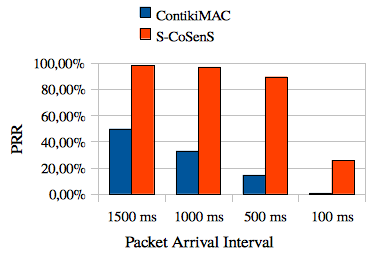
\includegraphics[width=8cm]{images/ch5-trp-8hz.png}
\flcaption{Résultats pour le taux de réception de paquets (PRR) pour un
cycle MAC~/ RDC de 8~Hz~/ 125~ms.}
\label{FigComparPRR8Hz}
\end{figure}

\begin{figure}[htb]
\centering
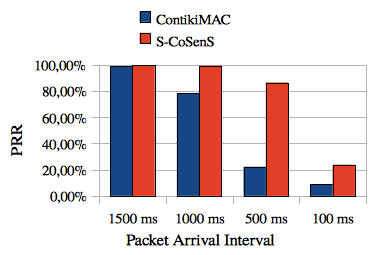
\includegraphics[width=8cm]{images/ch5-trp-16hz.png}
\flcaption{Résultats pour le taux de réception de paquets (PRR) pour un
cycle MAC~/ RDC de 16~Hz~/ 62~ms.}
\label{FigComparPRR16Hz}
\end{figure}

\begin{figure}[htb]
\centering
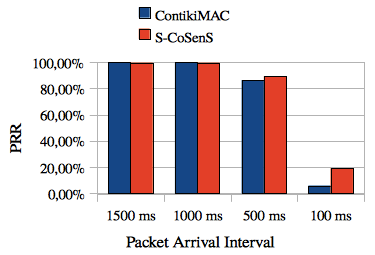
\includegraphics[width=8cm]{images/ch5-trp-32hz.png}
\flcaption{Résultats pour le taux de réception de paquets (PRR) pour un
cycle MAC~/ RDC de 32~Hz~/ 31~ms.}
\label{FigComparPRR32Hz}
\end{figure}

\begin{figure}[htb]
\centering
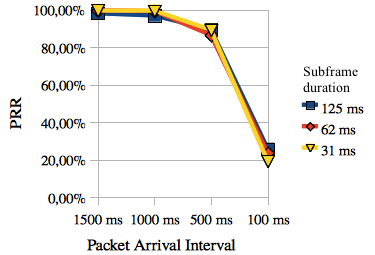
\includegraphics[width=8cm]{images/ch5-trp-stability-s-cosens.png}
\flcaption{Résultats combinés pour le taux de réception de paquets (TRP)
avec S-CoSenS, en fonction de la durée de la \lang{subframe}.}
\label{FigStablPRRSCoSenS}
\end{figure}

\begin{figure}[htb]
\centering
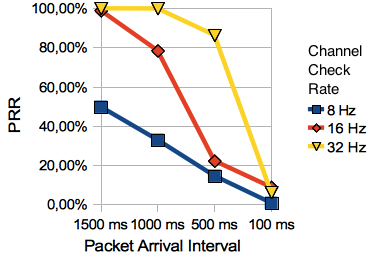
\includegraphics[width=8cm]{images/ch5-trp-unstability-contikimac.png}
\flcaption{Résultats combinés pour le taux de réception de paquets (TRP)
avec ContikiMAC, en fonction du \lang{channel check rate}.}
\label{FigInstablPRRContikiMAC}
\end{figure}

Les données représentées dans les figures \vrefrange{FigComparPRR8Hz}
{FigInstablPRRContikiMAC} nous montrent les faits suivants~:

\begin{itemize}

\item Le TRP de ContikiMAC augmente de façon significative avec le
\lang{channel check rate}, c'est-à-dire~: quand cet intervalle de
\lang{channel check rate} diminue, aboutissant à des cycles plus courts
et des écoutes plus fréquentes du médium radio.

\item Le TRP de S-CoSenS est toujours soit similaire, soit supérieur
à celui de ContikiMAC, quel que soit le scénario observé.

\item Le TRP de S-CoSenS reste très stable quelle que soit la valeur
donnée à la durée du cycle (\lang{subframe})~: cette stabilité est
clairement visible en figure \vref{FigStablPRRSCoSenS}. À l'inverse,
la figure \vref{FigInstablPRRContikiMAC} montre nettement que le TRP
de ContikiMAC varie énormément en fonction du \lang{channel check rate},
celui-ci devant être quadruplé (par rapport à sa valeur par défaut)
pour obtenir des résultats comparables à S-CoSenS.\\
Par conséquent, il est clair que les performances de S-CoSenS, en
matière de TRP, sont clairement plus prévisibles, et permettent de
s'assurer que le TRP restera dans des valeurs correctes ($> 80\%$)
dans la plupart des situations~--- c'est-à-dire tant que le médium
radio n'est pas complètement saturé comme dans le cas de notre
scénario <<~extrême~>>.

\end{itemize}

L'analyse détaillée des résultats des simulations, notamment le nombre
de retransmissions nécessaires pour chaque trame arrivé à destination,
nous montre également que~:

\begin{itemize}

\item avec ContikiMAC, les pertes de trames sont principalement dues
au routeur~;

\item avec S-CoSenS, le routeur ne perd jamais les trames qu'il a
reçus, toutes les pertes ont lieu lors des transmissions entre les
noeuds-feuilles et le routeur.

\end{itemize}

Cela n'est pas surprenant, car S-CoSenS réserve explicitement une période
de transmission (TP) durant chaque cycle exécuté par le routeur, pour
permettre à ce dernier de retransmettre les trames reçues dans les
meilleures conditions possibles. ContikiMAC ne possède lui aucune
fonctionnalité équivalente.

Durant ces périodes de transmission, une <<~priorité probabilistique~>>
est donnée par le protocole S-CoSenS aux routeurs, en leur accordant un
intervalle de base inférieur pour le calcul des périodes de \lang{backoff}
(il s'agit du paramètre nommé \emph{macMinBE} par le standard IEEE 802.15.4)
par rapport aux autres noeuds~: pour les routeurs $macMinBE = 2$, tandis que
pour les autres noeuds $macMinBE = 3$. Durant leurs périodes de transmission,
les routeurs sont ainsi privilégiés pour transmettre les trames présentes
dans leur file d'envoi.
Enfin et surtout, les noeuds-feuilles appartenant au même PAN qu'un routeur,
et ayant reçu ses \lang{beacons}, savent quand se déroule la période de
réception (WP) dudit routeur, et quand celle-ci s'achève pour laisser
la place à la période de transmission (TP). Les noeuds-feuilles appartenant
au même PAN que le routeur s'abstiennent alors de toute transmission,
remettant l'envoi des trames leur restant éventuellement à envoyer
au cycle suivant.

On peut clairement comprendre qu'au contraire, sous une forte charge
réseau, un routeur ContikiMAC va avoir des trames de données à recevoir
quasiment à chaque fois que celui-ci va sonder le médium radio
(\lang{``{Channel Check}''}) à chaque cycle. Ainsi, il va devenir de plus
en plus difficile pour ce routeur de trouver un intervalle disponible pour
l'envoi de ses propres trames au fur et à mesure que le trafic depuis les
noeuds-feuilles augmente. C'est pourquoi au cours de tels scénarios, le
noeud routeur devient clairement le point faible des PANs fonctionnant
sous ContikiMAC~; tandis que S-CoSenS peut éviter ces difficultés grâce
à sa conception, incluant une période de transmission (TP) réservée
à l'expédition des trames en attente dans la file d'envoi des routeurs.


\subsection{Délai total (<<~de bout-en-bout~>>) de transmission
            des trames}
\label{SubsecDelaiTransm}

Nous avons également calculé le délai que prend chaque trame transmise
avec succès pour aller de son noeud-feuille d'origine jusqu'au sink~---
c'est à dire la durée totale de son voyage en deux étapes
(\lang{``two-hop transmission''}). Ceci est le second indicateur de QdS
que nous avons étudié lors de ces expériences.

Les résultats que nous avons obtenus sont montrés dans les figures
\vrefrange{FigComparDelais8Hz}{FigInstablDelaisContikiMAC}.
Ces figures représentent les délais moyens nécessaires aux trames
transmises avec succès pour effectuer leur voyage en deux étapes. Notons que
les figures \vrefrange{FigComparDelais8Hz}{FigComparDelais32Hz}, pour des
raisons de lisibilité (tant la différence entre les résultats est énorme)
montrent les délais sur un axe vertical en échelle \emph{logarithmique}.

Contrairement aux résultats de TRP, ces résultats sont obtenus avec des
simulations où sont envoyés sans interruption des trames en nombre
indéfini, suivant là encore un intervalle moyen précalculé de transmission
entre deux trames consécutives. Le nombre de trames envoyées n'est donc
ici plus constant~; mais la charge générée sur le réseau reste fixée
de la même façon que pour les expériences sur le TRP.

\begin{figure}[htb]
\centering
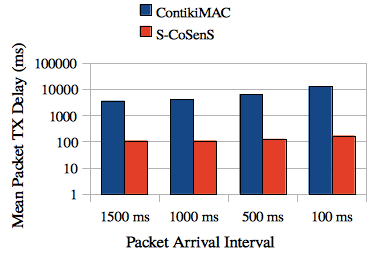
\includegraphics[width=8cm]{images/ch5-delays-8hz.png}
\flcaption{Résultats pour les délais moyens de transmission d'une trame
pour un cycle MAC~/ RDC de 8~Hz~/ 125~ms.}
\label{FigComparDelais8Hz}
\end{figure}

\begin{figure}[htb]
\centering
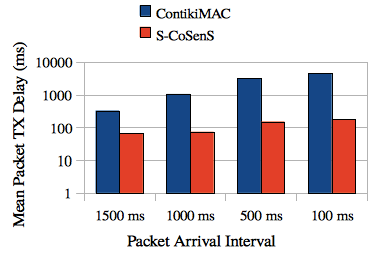
\includegraphics[width=8cm]{images/ch5-delays-16hz.png}
\flcaption{Résultats pour les délais moyens de transmission d'une trame
pour un cycle MAC~/ RDC de 16~Hz~/ 62~ms.}
\label{FigComparDelais16Hz}
\end{figure}

\begin{figure}[htb]
\centering
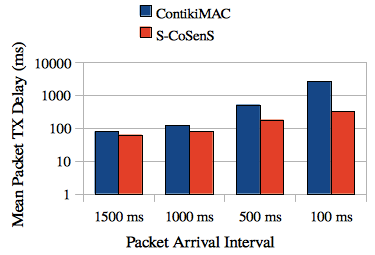
\includegraphics[width=8cm]{images/ch5-delays-32hz.png}
\flcaption{Résultats pour les délais moyens de transmission d'une trame
pour un cycle MAC~/ RDC de 32~Hz~/ 31~ms.}
\label{FigComparDelais32Hz}
\end{figure}

\begin{figure}[htb]
\centering
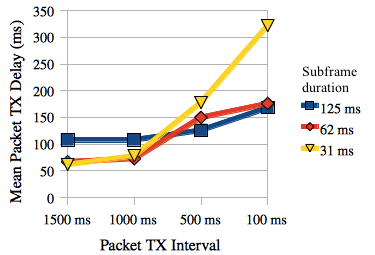
\includegraphics[width=8cm]{images/ch5-delays-stability-s-cosens.png}
\flcaption{Résultats combinés pour les délais moyens de transmission d'une
trame avec S-CoSenS, en fonction de la durée de la \lang{subframe}.}
\label{FigStablDelaisSCoSenS}
\end{figure}

\begin{figure}[htb]
\centering
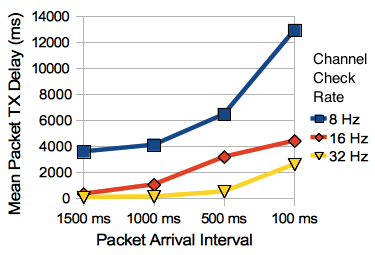
\includegraphics[width=8cm]{images/ch5-delays-unstability-contikimac.png}
\flcaption{Résultats combinés pour les délais moyens de transmission d'une
trame avec ContikiMAC, en fonction du \lang{channel check rate}.}
\label{FigInstablDelaisContikiMAC}
\end{figure}

\newpage

Ces résultats sur les délais de transmissions nous indiquent que~:

\begin{itemize}

\item Les délais de transmission sous ContikiMAC diminuent avec
l'augmentation du \lang{channel check rate}, c'est-à-dire~: quand 
les cycles ContikiMAC deviennent eux-mêmes plus courts.

\item Les délais de transmission sous S-CoSenS sont toujours soit
similaires, soit (dans la majorité des cas) nettement plus courts
que ceux de ContikiMAC, quel que soit le scénario observé.

\item Les délais de transmission sous S-CoSenS restent stables
quelle que soit la valeur donnée à la durée du cycle (\lang{subframe})~:
cette stabilité est clairement visible en figure
\vref{FigStablDelaisSCoSenS}. Dans la plupart des cas (c'est-à-dire
quand le médium radio n'est pas saturé), S-CoSenS permet de s'assurer
que les délais de transmission des trames resteront inférieurs à
une limite raisonnable (toujours $< 200$~ms, y compris dans les cas
les moins favorables).\\
À l'inverse, la figure \vref{FigInstablDelaisContikiMAC} montre
une instabilité énorme sous ContikiMAC dans les délais de transmission
en fonction des scénarios étudiés~: avec le réglage par défaut (8~Hz),
le délai de transmission des trames dépasse systématiquement et
largement le seuil de la seconde (plus de 12~secondes pour
transmettre une trame dans le cas le plus extrême).

\end{itemize}

On peut noter que ces trois observations (grande variabilité des résultats
de ContikiMAC, résultats similaires ou meilleurs pour S-CoSenS, stabilité
des résultats de S-CoSenS garantissant une QdS minimale) sont strictement
similaires à celles notées pour le taux de réception de paquets.

\bigskip

L'énorme augmentation dans les délais de transmission de bout-en-bout
pour ContikiMAC peut être interprétée comme un <<~excès de zèle~>>.
Une trame peut être transmise au cours d'un nombre prédéfini d'essais
(3~par défaut sous Contiki, 8~dans notre configuration par analogie
avec S-CoSenS). Rappelons que pour le couple ContikiMAC~-- CSMA/CA,
la transmission d'une trame peut être mise en attente jusqu'à la
disponibilité du médium radio, et qu'un <<~essai de transmission~>>
consiste à envoyer répétitivement cette trame jusqu'à concurrence
d'un cycle entier (durée calculée du \lang{channel check rate})~:
par conséquent, un délai énorme peut s'écouler avant que ce protocole
ne finisse par abandonner la transmission d'une trame donnée.

Si une telle <<~obstination~>> peut (en théorie) améliorer le TRP en
augmentant les chances de réception d'une trame par son destinataire,
elle finit par allonger de façon considérable le délai moyen pour la
transmission d'une trame de bout-en-bout. Au final, on peut s'interroger
sur l'utilité de continuer à chercher à transmettre des trames ayant
atteint un tel âge (dont les données risquent de devenir obsolètes),
souvent au détriment de la transmission de trames plus récentes
contenant des données plus actuelles donc plus utiles.

La configuration du nombre d'essais à tenter pour la transmission
d'une trame donnés est~--- comme pour de nombreux autres paramètres~---
un équilibre optimal à trouver entre deux buts contradictoires~: on
souhaite atteindre un TRP maximal, tout en permettant la perte et
l'élimination des trames trop âgées dont les données ont vraisemblablement
perdu leur intérêt. Il apparaît que dans les différents scénarios que nous
avons étudié, S-CoSenS permet d'obtenir un meilleur compromis entre
ces deux objectifs que ContikiMAC.


\subsection{Consommation d'énergie~: \lang{``Duty Cycles''}}
\label{SubsecDutyCycles}

Cooja peut facilement calculer les statistiques précises de \lang{``duty
cycle''}~--- ou pour être plus exact~: la fraction de temps pendant laquelle
les émetteurs~/ récepteurs radio sont actifs~--- pour chacune des
\lang{motes} virtuelles émulées. Ces statistiques sont un indicateur
très significatif pour quantifier les consommations d'énergie dans un
réseau de capteurs sans-fil, l'émetteur~/ récepteur radio étant, et de
loin, le circuit le plus gourmand en énergie au sein d'une \lang{mote}.

Les résultats obtenus pour les statistiques de \lang{duty cycle}
sont présentés dans les tables \vrefrange{TblDutyCyclesContikiMAC}
{TblDutyCyclesSCoSenS}. Notons qu'à cause des différences
importantes de TRP pour les durées de cycle de 125 et 62~ms, seule
la comparaison des résultats de \lang{duty cycle} pour des cycles de
31~ms avait un sens~; ce sont donc les seuls résultats que nous
présentons ici.

Dans ces deux tables, les lignes <<~activité radio~>> indiquent le
pourcentage du temps de simulation durant lequel l'émetteur~/ récepteur
accède activement au médium, et consomme donc de l'énergie.
Parmi ce temps d'activité, on distingue~:
\begin{itemize}
\item la fraction de temps durant laquelle le noeud émet avec succès
des trames de données (lignes <<~transmission efficace~>>)~;
\item la fraction de temps durant laquelle le noeud reçoit avec succès
des trames de données (lignes <<~réception efficace~>>)~;
\item la fraction de temps durant laquelle plusieurs noeuds émettent
simultanément, conduisant à la présence de signaux indéchiffrables sur
le médium radio (lignes <<~interférences~>>, qui couvrent en fait toutes
les émissions sans succès)~;
\item le temps d'activité radio n'étant pas couvert par ces trois
états précédents correspondent à des écoutes <<~à vide~>> du canal radio.
\end{itemize}


%%% ContikiMAC duty cycles
\begin{table}[htbp]
\centering
\begin{tabular}{|l|r|r|r|}
\hline
\multicolumn{4}{|c|}{ContikiMAC~: \lang{Channel Check Interval} = 32~Hz}\\
\hline
\multicolumn{4}{|r|}{INTERVALLE D'\'EMISSION DES TRAMES}\\
\hline
 & 1500 ms & 1000 ms & 500 ms \\
\hline
ROUTEUR                    & \multicolumn{3}{|c|}{ }\\
\hline
Activité radio             & 12,77\% & 17,85\% & 31,13\% \\
Transmission efficace      &  2,64\% &  4,00\% &  6,88\% \\
Réception efficace         &  2,78\% &  4,18\% &  8,24\% \\
Interférences              &  0,16\% &  0,40\% &  2,64\% \\
\hline
 NOEUDS-FEUILLES (moyenne) & \multicolumn{3}{|c|}{ }\\
\hline
Activité radio             &  5,61\% &  7,45\% & 14,27\% \\
Transmission efficace      &  0,90\% &  1,48\% &  3,89\% \\
Réception efficace         &  0,66\% &  1,03\% &  1,96\% \\
Interférences              &  0,11\% &  0,21\% &  1,13\% \\
\hline
\end{tabular}
\flcaption{Statistiques de \lang{duty cycle} pour ContikiMAC.}
\label{TblDutyCyclesContikiMAC}
\end{table}


%%% S-CoSenS duty cycles
\begin{table}[hbtp]
\centering
\begin{tabular}{|l|r|r|r|}
\hline
\multicolumn{4}{|c|}{S-CoSenS~: Durée d'un cycle (\lang{subframe}) = 31~ms}\\
\hline
\multicolumn{4}{|r|}{INTERVALLE D'\'EMISSION DES TRAMES}\\
\hline
 & 1500 ms & 1000 ms & 500 ms \\
\hline
ROUTEUR                    & \multicolumn{3}{|c|}{ }\\
\hline
Activité radio             & 66,22\% & 67,56\% & 67,91\% \\
Transmission efficace      &  4,96\% &  5,48\% &  8,43\% \\
Réception efficace         &  3,84\% &  4,43\% &  8,90\% \\
Interférences              &  1,04\% &  1,48\% &  8,39\% \\
\hline
 NOEUDS-FEUILLES (moyenne) & \multicolumn{3}{|c|}{ }\\
\hline
Activité radio             &  6,15\% &  7,68\% & 40,04\% \\
Transmission efficace      &  0,58\% &  0,70\% &  2,64\% \\
Réception efficace         &  0,68\% &  0,93\% &  7,08\% \\
Interférences              &  0,16\% &  0,22\% &  3,98\% \\
\hline
\end{tabular}
\flcaption{Statistiques de \lang{duty cycle} pour S-CoSenS.}
\label{TblDutyCyclesSCoSenS}
\end{table}


Les statistiques de \lang{duty cycle} présentées dans les tables
\vrefrange{TblDutyCyclesContikiMAC}{TblDutyCyclesSCoSenS} indiquent de
façon évidente que ContikiMAC possède sur ce terrain un avantage
très significatif. Les taux d'activité radio, que ce soit en émission,
en réception, ou en attente, sont toujours plus faibles~--- c'est à dire
meilleurs~--- pour ContikiMAC que pour S-CoSenS. Cela est particulièrement
vrai pour l'activité radio globale sur les noeuds routeurs, où la
différence en faveur de ContikiMAC est proprement spectaculaire.
(Cette différence est surtout due à la nécessité de fixer
$\mathrm{WP}_{min}$ à 50\% pour estimer correctement le trafic radio~---
cf. section \vref{SubSecPropoAlgo}.)
Ces constatations sont illustrées par les figures
\vrefrange{FigDutyCyclesRouteurs}{FigDutyCyclesFeuilles}.


%% figures de comparaison des "duty-cycles" pour les routeurs
\begin{figure}[htbp]
\centering
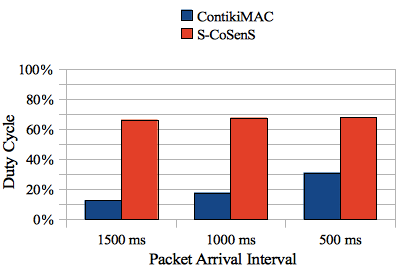
\includegraphics[width=8cm]{images/ch5-duty-cycles-routeurs.png}
\flcaption{Comparaison de l'activité radio (\lang{duty cycle}) sur les
noeuds routeurs fonctionnant respectivement sous ContikiMAC et S-CoSenS,
avec des \lang{subframes} de 31~ms.}
\label{FigDutyCyclesRouteurs}
\end{figure}


%% figures de comparaison des "duty-cycles" pour les noeuds-feuilles
\begin{figure}[htbp]
\centering
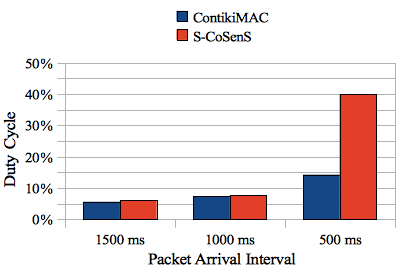
\includegraphics[width=8cm]{images/ch5-duty-cycles-noeuds-feuilles.png}
\flcaption{Comparaison de l'activité radio (\lang{duty cycle}) sur les
noeuds-feuilles fonctionnant respectivement sous ContikiMAC et S-CoSenS,
avec des \lang{subframes} de 31~ms.}
\label{FigDutyCyclesFeuilles}
\end{figure}


ContikiMAC prouve ainsi qu'il est en effet \emph{un protocole à très
basse consommation d'énergie}.

\bigskip

La seule exception à cette constatation de supériorité générale de
ContikiMAC en matière de \lang{duty cycle} se situe dans les temps
d'émission (lignes <<~transmission efficace~>>)~: pour les
noeuds-feuilles~--- mais \emph{pas} pour les routeurs~--- les \lang{duty
cycles} sont systématiquement légèrement inférieurs (c-à-d. meilleurs)
pour S-CoSenS. Cela s'explique aisément par la conception de ces deux
protocoles~: S-CoSenS est conçu~--- pour les transmissions entre
noeuds-feuilles et routeur~--- sur le paradigme RI-LPP (cf. section
\vref{SubsecProtoMACLPP}), ce qui implique naturellement moins de
tentatives de transmissions de trames de données que pour ContikiMAC
qui est conçu sur le paradigme LPL (cf. section \vref{ParContikiMAC})~---
et plus spécifiquement sur l'envoi continu de trames de données entières
par l'émetteur jusqu'à acquittement par le destinaire.


\subsection{Stabilité et contraintes mémoire}
\label{SubsecStabl}

Durant le développement et l'évaluation de S-CoSenS, nous avons
fait face à plusieurs plantages, notamment lorsque nous avons tenté
d'utiliser de longues files d'envoi de trames. Ces plantages étaient
dûs aux débordements de la pile système qui empiétait sur l'espace mémoire
de cette file~: quand cette dernière était pleine, les données des trames
pouvaient ainsi écraser le contenu de la pile système (lorsque ladite pile
contenait une quantité de données dépassant son espace mémoire alloué),
aboutissant bien évidemment à des erreurs logicielles fatales.

Les plantages observés avec cette implantation de S-CoSenS sous RIOT sont
dûs à la quantité très limitée de RAM disponible pour les données (8~Ko)
dans le microcontrôleur MSP430 autour duquel est bâtie la \lang{mote}
Zolertia Z1. Ceci, combiné à l'absence d'unité de protection mémoire
(MPU) dans cette architecture matérielle, aboutit à la survenue de
problèmes de corruption mémoire silencieux et indétectables en temps
voulu.

Si l'utilisation de microcontrôleurs disposant d'une quantité de RAM plus
conséquente peut limiter la survenue de tels problèmes, la détection
systématique de ces derniers et leur traitement correct nécessite
l'un des mécanismes suivants~:

\begin{enumerate}

\item \emph{Un mécanisme matériel} destiné à détecter les accès mémoire
incorrects et à provoquer une exception au début de leur survenue, avant
leur réalisation effective, prévenant ainsi leurs conséquences~: au sein
d'un microcontrôleur, ceci est le rôle d'une \nom{MPU} (\lang{Memory
Protection Unit}). Certaines architectures (comme les ARM Cortex-M)
proposent en option une telle fonctionnalité. Celle-ci nous semble
indispensable pour la conception de systèmes destinés à offrir un niveau
minimal de sûreté de fonctionnement (\lang{``safe systems''}).

\medskip

\item Pour les architectures dépourvues de MPU, \emph{un système de
support logiciel} dont le rôle est de surveiller les valeurs de registres
critiques~--- tels que le pointeur de pile (\nom{SP}~: \lang{Stack
Pointer})~--- ne serait-ce que pour s'assurer que ces valeurs restent
comprises au sein d'intervalles autorisés.\\
Un tel mécanisme peut être implanté \emph{au niveau d'un système
d'exploitation} (FreeRTOS et RIOT fournissent une telle option)~;
mais ce mécanisme ne peut~--- sans le support matériel d'une MPU~--- que
vérifier et constater la présence ou non d'une violation d'espace mémoire,
et en aucun cas empêcher sa survenue et ses conséquences. En cas de problème,
la seule alternative possible reste d'arrêter le système, et de le faire
éventuellement redémarrer <<~à froid~>> (\lang{``hard reset''}).\\
Un moyen plus efficace serait \emph{d'ajouter automatiquement, au cours du
processus de compilation, des séquences de code de vérification,} notamment
pour surveiller l'évolution de la valeur du registre SP lors de l'entrée
dans un sous-programme ou~--- pour les environnements multitâches~---
lors d'un changement de contexte. Ces types d'évènements étant ceux
augmentant la taille de la pile, ils correspondent donc aux moments
où cette dernière risque de déborder de son espace réservé.
Il deviendrait alors possible (comme avec une MPU) d'implanter un
traitement spécifique préventif des erreurs mémoires, n'interrompant que
les tâches ou routines fautives, sans devoir arrêter le système entier.

\end{enumerate}

\bigskip

Pour nos présentes expérimentations, nous avons contourné le problème
en réduisant simplement la profondeur de notre file d'envoi de trames,
laissant ainsi une place suffisante à la pile système.

\bigskip

Notons enfin que ce problème n'est nullement spécifique à RIOT ni à aucun
système d'exploitation embarqué, mais peut toucher tous les OS fonctionnant
sur du matériel aux ressources limitées, et surtout dépourvu d'une MPU ou
d'un autre mécanisme matériel de protection de la mémoire. Citons par
exemple \cite{ContikiPort8051} où sont expliquées les difficultés de portage
de Contiki sur une plate-forme matérielle courante et aux ressources
limitées~: on y parle clairement des problèmes de débordement de pile
(voir par exemple la figure~1 de cette publication), et des optimisations
qui ont été nécessaires pour éviter ce problème.

La stratégie de conception de systèmes extrêmement peu gourmands en
ressources comme Tiny OS et Contiki est de pousser l'optimisation à
l'extrême pour limiter ces problèmes au maximum (sans pour autant pouvoir
garantir une fiabilité absolue).


\subsection{Influence de l'optimisation des implantations}
\label{SubsecOptim}

Lors de nos différents tests, nous avons constaté que les délais
observés pour charger les trames dans le \lang{buffer} d'envoi du
composant radio CC2420 étaient toujours significativement plus longs
sous RIOT OS que sous Contiki.

Nos investigations à ce sujet nous ont montré que ces importantes
différences de délai étaient dues à la façon dont la communication
sur le bus SPI~--- assurant le lien entre le microcontrôleur central
et l'émetteur~/ récepteur radio dans la \lang{mote} utilisée~--- est
gérée par le système d'exploitation. Sous RIOT OS, lorsqu'un octet est
transmis sur le bus SPI, le résultat de la transmission est toujours
attendu, en consultant les \lang{flags} indiquant le succès ou l'échec,
avant de transmettre l'octet suivant. À l'inverse, Contiki utilise une
procédure nommée \lang{``fast SPI write''} envoyant un octet sur le bus
SPI dès que ce dernier est disponible (c'est-à-dire que le registre
d'envoi de l'interface microcontrôleur du bus SPI est disponible en
écriture), sans attendre de connaître le résultat de la transmission
précédente (les \lang{flags} indiquant le résultat d'une transmission
prenant un certain temps pour se mettre à jour).

Si la solution utilisée par Contiki est clairement plus rapide, elle
est également peu sûre car incapable de détecter correctement un
problème pouvant survenir sur le bus SPI~; l'implantation de
RIOT est au contraire sûre, mais plus lente.

Il y a clairement ici un compromis entre optimisation des performances
et fiabilité. Pour le chargement du \lang{buffer} d'envoi de l'émetteur~/
récepteur radio CC2420, cela dépend en fait moins de l'OS lui-même que
des choix d'implantation pour le pilote du bus SPI.


\begin{table}[!htb]
\centering
\begin{tabular}{|l|r|r|}
\hline
Système / Pilote SPI &  \multicolumn{2}{|c|}{Délai chargement} \\
\hline
RIOT OS~/ Standard (Sûr)            & 89 ticks & 2716 $\mu$s \\ 
RIOT OS~/ \lang{``Fast SPI write''} & 36 ticks & 1099 $\mu$s \\
Contiki~/ \lang{``Fast SPI write''} & 14 ticks &  213 $\mu$s \\
\hline
\end{tabular}
\flcaption{Delais observés pour le chargement d'une trame de 110 octets
dans le \lang{buffer} d'envoi de la radio CC2420 d'une \lang{mote} Zolertia
Z1, en fonction de l'OS et de l'implantation du pilote SPI.}
\label{TblTXPktLoadDelays}
\end{table}


Nous avons implanté l'optimisation \lang{``fast write''} du pilote SPI
sous RIOT, et avons mesuré les différences de rapidité entre
les deux versions du pilote sous RIOT, ainsi qu'avec le pilote
standard de Contiki. Les résultats sont montrés en table
\vref{TblTXPktLoadDelays}.

Les délais dans la table \vref{TblTXPktLoadDelays} sont donnés
dans la deuxième colonne en \lang{``ticks''} de \texttt{rtimer/hwtimer}
\footnotemark[2], les deux s'incrémentant à la fréquence de 32768~Hz.
Le \lang{``tick''} est donc une unité de temps fixe égale à environ
30,5 microsecondes. Les valeurs correspondantes en microsecondes sont
données en troisième colonne pour plus de facilité.

\footnotetext[2]{Rappelons que \texttt{rtimer} est le mécanisme de gestion
de \lang{timer} matériel en temps réel de Contiki OS, dont nous avons décrit
les limitations en section \vref{SubsecContikiTempsReel}~; \texttt{hwtimer}
est le mécanisme équivalent, plus performant, que nous avons utilisé sous
RIOT OS. Cependant, comme nous l'avons vu en section \vref{SubsecRIOTOS},
\texttt{hwtimer} a depuis été remplacé par le module \texttt{xtimer}.}

Nous pouvons quoi qu'il en soit noter que la pénalité imposée à S-CoSenS
par le pilote SPI standard de RIOT ne l'a pas empêché d'obtenir des
performances supérieures en matière de QdS (tous les tests faits avec
RIOT décrits dans la présente section ayant été exécutés avec le
pilote SPI standard du système).

\bigskip

Notons par contre que, contre toute attente, les délais de chargement
obtenus par simulation sous Cooja~/ MSPSim, montrés en table
\vref{TblTXPktLoadDelays} diffèrent très largement de ceux obtenus
sur une \lang{mote} Zolertia Z1 réelle. Nous reviendrons en détail sur ce
phénomène dans la section \vref{SecLimInexactSimu} du prochain chapitre.

Ce phénomène étonnant nous a en outre poussé à tenter de reproduire,
au moins partiellement, nos expériences sur matériel réel. C'est le sujet
de la section \ref{SubsecExpMat} suivante.


\subsection{Comparaison avec essais sur matériel}
\label{SubsecExpMat}

En nous basant sur les résultats obtenus dans la présente section
\ref{SecEvalPerfSCosens}, nous avons constaté que S-CoSenS avait
l'avantage sur ContikiMAC concernant les critères de QdS (TRP et délais
de transmission). Inversement, ContikiMAC est supérieur à S-CoSenS
concernant les \lang{duty cycles} (et donc la consommation d'énergie).

Les précédentes expériences ont bien sûr leurs limitations, la principale
d'entre elles étant qu'il s'agit uniquement de simulations. Cela peut
entraîner des inexactitudes et, à l'extrême, des conclusions erronées,
comme nous le verrons ultérieurement en section \vref{SecLimInexactSimu}.

Pour tenter de valider ces résultats de simulations, nous avons effectué
quelques tests sur un ensemble de noeuds WSN430 d'IoT-LAB. IoT-LAB
\cite{IotLAB} est un banc d'essai matériel permettant d'effectuer des tests
à distance sur des milliers de \lang{motes} de différents types~; nous
en reparlerons plus largement au chapitre \vref{ChValidation}.

Les \lang{motes} WSN430 que nous avons utilisées sont similaires aux
TelosB~/ SkyMotes (elles sont notamment basées sur le MSP430F1611),
et non à la Zolertia Z1 (construite autour d'un MSP430F2617, cf. section
\vref{SecHWMSP430})~; les conditions d'expérimentation ne sont donc
pas strictement similaires, mais sont destinées à nous donner une idée
générale de la validité de nos simulations.

Nous avons repris un PAN dont la structure est similaire à celle présentée
en figure \vref{FigVirtualPAN1}. Bien évidemment, il s'agit désormais
dans ces nouveaux tests de matériel réel.

Nous nous sommes limités à deux jeux d'essais, consistant à tester
l'implantation de S-CoSenS sous RIOT, avec deux durées de \lang{subframe}~:
\begin{itemize}
\item une durée de \lang{subframe} égale à 125~ms, correspondant à la
configuration de nos premiers jeux de simulation~;
\item une durée de \lang{subframe} égale à 100~ms~--- donc intermédiaire
entre les deux premières valeurs simulées~--- pour essayer d'avoir une
idée de l'évolution en allant vers des valeurs de \lang{subframe}
inférieures, comme pour les simulations.
\end{itemize}

Les résultats que nous avons obtenus avec nos expériences sur matériel
réel pour les taux de réception de paquets sont présentés en figure
\vref{FigPRRIoTLAB}.

\begin{figure}[htb]
\centering
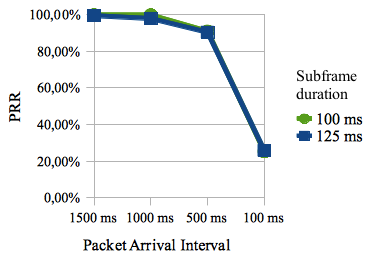
\includegraphics[width=8cm]{images/ch5-trp-iot-lab.png}
\flcaption{Résultats obtenus pour le taux de réception de paquets (TRP)
avec S-CoSenS, en fonction de la durée de la \lang{subframe}, sur des
\lang{motes} IoT-LAB WSN430.}
\label{FigPRRIoTLAB}
\end{figure}

\bigskip

On voit que les courbes présentées sont tout à fait similaires
à celles obtenues par simulation, telles que montrées dans la figure
\vref{FigStablPRRSCoSenS}, et semblent donc valider globalement
nos travaux et conclusions pour le TRP de notre protocole.

\smallskip

Concernant les délais de transmission, les résultats des expériences
sur matériel sont visibles en figure \vref{FigDelaisIoTLAB}.

\begin{figure}[htb]
\centering
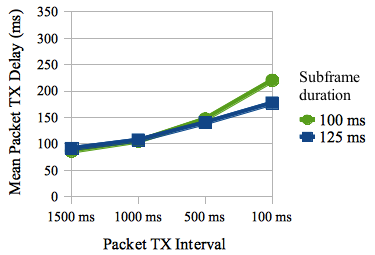
\includegraphics[width=8cm]{images/ch5-delays-iot-lab.png}
\flcaption{Résultats obtenus pour les délais moyens de transmission d'une
trame avec S-CoSenS, en fonction de la durée de la \lang{subframe}, sur
des \lang{motes} IoT-LAB WSN430.}
\label{FigDelaisIoTLAB}
\end{figure}

Notons ici que les délais, pour les simulations, étaient calculés très
précisément grâce à la fonction de relevé temporel des trames circulant
sur le média radio virtuel offerte par Cooja (fenêtre \lang{``Radio
messages''} et ses données exportables sous forme de fichier CSV).
Les motes WSN430 d'IoT-LAB ne possédant pas de \lang{``sniffers''}
de trames, les délais obtenus par ces tests sur matériel sont calculés
à partir de traces (\lang{``logs''}) de déboguage émises par les noeuds
utilisés lors de ces tests. Ces opérations d'écriture de traces (fonctions
de la famille \texttt{*printf()}) prenant elles-mêmes un certain temps
d'exécution, cela représente un biais supplémentaire entre ces expériences
sur matériel et nos simulations (en plus de la différence de
microcontrôleur).

Cela dit, les courbes nous montrent là encore des valeurs du même ordre
que celles obtenues par simulation en figure \vref{FigStablDelaisSCoSenS}.
Nos travaux et conclusions pour les délais de transmissions de notre
protocole semblent donc eux aussi valides.

\medskip

Nous n'avons par contre aucune donnée de \lang{``duty cycle''} issue de
ces expériences sur matériel à fournir, les motes WSN430 étant comme nous
l'avons dit dépourvues de l'instrumentation adéquate~--- alors que Cooja
fournit une fonction de calcul automatique de ces \lang{``duty cycles''}
via sa fenêtre \lang{``Timeline''}. Nous ne pouvons donc valider ou
invalider nos données simulées de \lang{``duty cycle''} via les présents
jeux d'expériences sur matériel.

%%%%%%%%%%%%%%%%%%%%%%%%%%%%%%%%%%%%%%%%%%%%%%%%%%%%%%%%%%%%%%%%%%%%%%%%%%%%%

\section{Améliorations potentielles des protocoles MAC~/RDC}
\label{SecAmeliorAlgoProtoMAC}


\subsection{Propositions d'améliorations algorithmiques}
\label{SubSecPropoAlgo}

Là encore, il s'agit de trouver un équilibre entre les deux objectifs
contradictoires que sont l'obtention d'une QdS maximale et de \lang{duty
cycles} minimaux. Par conception, ContikiMAC est clairement plus orienté
vers le second objectif que S-CoSenS, même s'il est possible de diminuer
la valeur du paramètre $\mathrm{WP}_{min}$ pour pousser notre protocole
à se rapprocher du même objectif. Cela est toutefois contraire à notre
politique consistant à donner la priorité absolue à la QdS.

Nous avons également, au cours de ces expériences, été amenés à réfléchir
sur les possibilités d'amélioration et d'optimisation de notre protocole
S-CoSenS, puis plus généralement de tout protocole MAC~/ RDC à haute
performance~:

\begin{enumerate}

\item En premier lieu, l'observation de ContikiMAC et de son fonctionnement
nous a poussé à \emph{tenter d'implanter un mécanisme similaire à
l'optimisation \lang{``phase lock''} de ContikiMAC (discutée en section
\vref{ParContikiMAC})} afin d'obtenir des \lang{duty cycles} inférieurs~---
c-à-d. meilleurs~--- pour les noeuds-feuilles fonctionnant sous S-CoSenS.

Les résultats de nos essais de simulation avec une telle optimisation se
sont révélés relativement concluants sous certaines conditions, comme
expliqué dans la section \ref{SubSecEvalAlgoSimu} suivante.

Plus qu'avec S-CoSenS, \emph{cette optimisation peut surtout être mise
à profit pour améliorer tout protocole asynchrone}, pour ajuster au mieux
les moments d'activation de la radio pour tenter d'émettre (protocoles LPL)
ou recevoir (protocoles LPP) des trames, \emph{si le protocole en question
possède une durée de cycle constante (ou au minimum prévisible).}

\smallskip

\item Une autre amélioration que nous avons imaginée pour S-CoSenS est
la suivante~: au lieu de compter le nombre de paquets retransmis par le
routeur durant les cycles précédents pour évaluer le trafic radio et
calculer la durée des périodes d'écoute WP (cf. section \vref{ParSCoSenS}),
nous souhaitons désormais nous servir du nombre de \nom{SFD} \footnotemark[3]
entendus durant les périodes d'écoute précédentes pour mieux évaluer
le trafic réseau passant et donc calculer plus justement les durées
des périodes d'écoute suivantes.

\footnotetext[3]{\nom{SFD~: \lang{``Start of Frame Delimiter''}}~;
il s'agit d'un signal radio (de contenu constant, prédéfini par la couche
physique du standard IEEE 802.15.4) envoyé sur le médium comme marqueur
pour signaler le début de l'émission d'une trame, et permettre la
synchronisation des récepteurs radio pour la bonne réception de cette
nouvelle trame.}

\smallskip

Comme nous l'avons vu dans la section \vref{ParSCoSenS} de l'état de l'art,
S-CoSenS (dans sa version actuelle) partage ses \lang{``subframes''} de
longueur fixe entre une période d'écoute WP et une période de sommeil SP.
Le calcul de la durée de WP est actuellement effectué sur la base du
nombre de trames reçues avec succès durant les périodes d'écoutes des
cycles précédents (via une moyenne glissante).

\smallskip

Ce mécanisme est efficace en théorie, mais ne tient pas compte du bruit.
Un réseau sans-fil peut être parasité par de nombreux facteurs
(interférences, collisions, ou même trames destinées à d'autres noeuds
surtout si plusieurs PANs différents sont présents à proximité).

En présence d'un tel bruit, les trames destinées à un noeud $N$ vont
être <<~noyées~>> dans la masse de signaux sans intérêt pour ce noeud $N$.
Par conséquent, avec le mode de calcul actuel, le noeud $N$, recevant peu
de trames utiles, va diminuer rapidement sa période d'écoute WP (passant
ainsi la majorité de ses cycles en période de sommeil SP). Il arrivera
alors, dans un milieu fortement bruité, que le noeud $N$ manque ainsi
des trames lui étant destinées. C'est pour cela que nous avons dû fixer
$\mathrm{WP}_{min}$ à 50\% sur les routeurs S-CoSenS lors de nos tests
(cf. section \vref{SubsecDutyCycles}) afin d'assurer une QdS suffisante.
(Nous donnons priorité absolue à la QdS~: voir la conclusion en section
\vref{SecDiscussContribConcluProtocolesMAC}).

Nous nous proposons, pour calculer la durée de WP, de ne plus compter le
nombre de trames reçues avec succès, mais de compter le nombre de SFD reçus,
c'est-à-dire le nombre de trames détectées sur le médium radio. Un tel
mode de calcul permet de tenir compte de tout le trafic <<~normal~>>
sans pour autant prendre en compte le <<~bruit brut~>> (interférences,
signaux non conformes au protocole IEEE 802.15.4)~; cela devrait ainsi
permettre à un noeud $N$ d'éviter de manquer des trames lui étant
destinées, pour cause de WP trop courte. Le défaut potentiel de cette
technique est d'augmenter la durée de WP, donc mécaniquement de diminuer
celle de SP, c'est-à-dire d'augmenter la consommation d'énergie du noeud,
peut-être inutilement. 

La contribution attendue de ces tests sur matériel réel est donc de
\emph{comparer les deux modes de calcul de la durée de WP~--- nombre
de trames reçues, et nombre de SFD détectés~--- et de déterminer par
l'expérience lequel représente le meilleur compromis} entre QdS (nombre
de trames reçues ou manquées) et consommation d'énergie (durée optimale
ou non de la période de sommeil SP).

Notons également que \emph{le recours aux SFD pour évaluer l'intensité
du trafic réseau peut être mis à profit pour améliorer tout protocole
ayant besoin de connaître cette intensité~--- ou même pouvant faire usage
de cette information~--- pour adapter dynamiquement son fonctionnement}.
ContikiMAC pourrait par exemple s'en servir pour faire varier de façon
dynamique son \lang{Channel Check Interval} en fonction du trafic,
l'augmentation de la fréquence de ce paramètre permettant visiblement
de mieux traiter les charges réseau intenses.

\item Nous avons également eu l'idée de combiner nos tests avec une
\emph{évaluation de l'influence du seuil de réception de l'émetteur~/
récepteur radio (\lang{``CCA Threshold''})}, telle qu'étudiée en détail
dans une publication de 2013 \cite{CCAThresholdStudy}~--- proposant un
protocole nommé \nom{AEDP} (\lang{``Adaptive Energy Detection Protocol''})
permettant d'améliorer la fiabilité des liens réseaux face au bruit
présent sur le médium radio~---, pour une éventuelle inclusion de la
gestion du \lang{``CCA Threshold''} dans la pile réseau de notre
plate-forme logicielle.

Le protocole AEDP décrit en \cite{CCAThresholdStudy} se penche sur
le problème du bruit, et de l'activité inutile des émetteurs~/ récepteurs
radio qui en découle.

Son principe est, pour résumer, d'adapter le seuil de sensibilité en dBm
de la radio (\lang{``CCA Threshold''}) en fonction de deux variables~:
le nombre d'envois nécessaires d'une trame donnée pour que celle-ci puisse
être transmise avec succès (variable ${ETX}$), et le nombre d'activations
de la radio nécessaires pour pouvoir détecter l'arrivée d'un signal utile
(variable ${WR}$). Le protocole AEDP consiste à ajuster le \lang{``CCA
Threshold''} (ici nommé variable $T$) tout en gardant $ETX$ en dessous
d'une valeur maximale d'essais pour réussir à envoyer une trame (constante
${ETX}_{threshold}$)~--- ce qui implique de diminuer $T$~---, \emph{et} en
évitant que $WR$ ne dépasse une valeur maximale correspondant au nombre
estimé nécessaire d'activations de la radio pour une réception correcte
(constante ${WR}_{threshold}$)~--- ce qui implique de d'augmenter $T$. \\
Pour résumer, le but du protocole AEDP est de trouver la valeur minimale
de $T$ telle que ${ETX} < {ETX}_{threshold}$ et ${WR} < {WR}_{threshold}$.
On voit qu'il s'agit, une fois de plus, d'un compromis entre QdS (taux
de réception de trames et débit de données: $ETX$) et consommation
minimale d'énergie ($WR$).

Ce protocole a au départ été conçu pour les protocoles LPL, dont le principe
est rappelons-le de se réveiller à intervalles (plus ou moins) réguliers
pour vérifier si une trame leur est destinée~--- cf. section
\vref{SubsecProtoMACLPL} de l'état de l'art~---, et a été testé
par ses auteurs sur TinyOS et Contiki.

Bien que S-CoSenS ne repose pas principalement sur LPL, le principe
consistant à jouer sur le \lang{``CCA Threshold''} pour améliorer le
rapport signal~/ bruit (\nom{SNR}~: \lang{Signal/Noise Ratio}) est
intéressant et peut être complémentaire, pour S-CoSenS, de l'essai
de la méthode du comptage des SFD pour optimiser le rapport QdS~/
consommation d'énergie.

On peut raisonnablement penser que \emph{l'adaptation dynamique du
\lang{``CCA Threshold''} pour améliorer le rapport signal~/ bruit peut être
mise à profit par n'importe quel protocole MAC~/ RDC~--- voire même plus
directement au niveau des pilotes radio eux-mêmes~--- pour améliorer les
performances et l'efficacité des transmissions sur les réseaux sans-fil}.

\end{enumerate}


\subsection{\'Evaluation de ces propositions~: difficultés et
            inadéquation des simulations}
\label{SubSecEvalAlgoSimu}

Il est naturel, pour tenter une première évaluation des trois
propositions d'améliorations algorithmiques détaillées dans la section
\ref{SubSecPropoAlgo} précédente, de songer à effectuer des simulations
utilisant des scénarios adéquats (notamment avec le \lang{framework} Cooja~/
MSPSim que nous avons déjà largement utilisé).

Toutefois, il s'avère que la mise en place de tels scénarios pour effectuer
des simulations~/ émulations valides est problématique, pour les raisons
suivantes~:

\begin{enumerate}

\item Concernant \emph{l'implantation d'un mécanisme similaire à
l'optimisation \lang{``phase lock''} de ContikiMAC}, notre but est
d'obtenir des données de \lang{``duty cycle''} afin de vérifier si des
améliorations significatives~--- c.-à-d. des valeurs d'activité radio
significativement inférieures~--- peuvent être obtenues. Or, comme nous
l'avons évoqué en section \vref{SubsecOptim}, et comme nous l'étudierons
en détail en section \ref{SecLimInexactSimu} au chapitre suivant, les
résultats (notamment de \lang{``duty cycle''}) obtenus à l'aide du
\lang{``framework''} Cooja~/ MSPSim manquent de fiabilité.
\emph{Les conclusions sur les éventuelles améliorations obtenues par
l'implantation du mécanisme de \lang{``phase lock''} via une étude faite
par simulations~/ émulations ne seront donc pas robustes, et pourront
facilement être remises en question}.

\item Concernant \emph{l'étude de l'influence des SFD sur le calcul de la
durée de la période d'écoute WP de S-CoSenS}, le matériel émulé par Cooja~/
MSPSim~--- à savoir les \lang{motes} Sky~/ TelosB tout comme les Z1~---
ne permet pas de recevoir l'interruption correspondant aux SFD (début de
réception d'une trame) de façon simple~: ces différentes \lang{motes}
relient en effet cette interruption à une entrée (\lang{``capture''}) d'un
des \lang{timers} du microcontrôleur central. Il faudrait pour la détecter
effectuer des modifications complexes et non portables au mécanisme de
gestion des \lang{timers} de RIOT, ce qui nuirait probablement à la
fiabilité de ce dernier. Une étude mettant en place une version ainsi
<<~altérée~>> de RIOT, d'une qualité insuffisante, n'aurait que peu
d'intérêt car ne pouvant fournir une implantation robuste et pérenne.
Il existe des \lang{motes} permettant de recevoir et gérer facilement
(du moins au niveau physique) les interruptions liées aux SFD, mais toutes
celles que nous connaissons sont des plates-formes matérielles basées sur
l'architecture ARM, pour laquelle aucun émulateur efficace n'est à l'heure
actuelle reconnu comme fiable, disponible et compatible avec Cooja.
\emph{Il nous est donc impossible d'émuler~--- du moins avec le
\lang{``framework''} Cooja~/ MSPSim que nous avons jusqu'ici utilisé~---
un matériel permettant de détecter les SFD de manière fiable et efficace.}

\item Concernant \emph{l'étude de l'influence du rapport signal~/ bruit
(SNR) sur l'optimisation de la qualité de service et la consommation
d'énergie}, une telle étude implique~--- par nature~--- le médium radio
de façon centrale. Or, il est bien connu que la simulation du médium radio
est le point faible de toutes les études par simulation des réseaux
sans-fil (qu'il s'agisse des WSN comme des réseaux plus <<~classiques~>>
comme le WiFi). En effet, comme nous l'avons vu notamment au chapitre
\ref{ChCtxProb}, le médium radio est par nature peu fiable, sujet à la
diffusion et présente des variations fortes et rapides~--- le plus souvent
imprévisibles~--- en fonction du temps et de l'espace. \emph{Des études
du SNR par simulation sont donc vouées à avoir une fiabilité, et donc
un intérêt, extrêmement limités.}

\end{enumerate}

\smallskip

\emph{Nous voyons donc que sur nos trois propositions d'améliorations
algorithmiques, les deux dernières ne peuvent pas être étudiées de façon
assez fiable par simulation~/ émulation}, et nécessiteront donc des études
sur des réseaux réels. Nous avons fourni une contribution mettant en place
la fonctionnalité de gestion du \lang{``CCA Threshold''} \cite{PRriotEnh13}
(nécessaire par exemple au protocole AEDP), qui pourra ainsi faire l'objet
de travaux ultérieurs idoines.

\smallskip

\emph{Concernant la première amélioration (\lang{``phase lock''}), une
étude par simulation, si elle n'offre pas une fiabilité satisfaisante,
est néanmoins possible pour tenter de se faire une première idée grossière
de l'efficacité d'une telle optimisation} (qui demandera bien sûr par la
suite confirmation par des tests sur matériel réel). Nous avons donc exécuté
un jeu de simulations, dans cette optique bien limitée d'exploration
préliminaire.

Nous avons repris le scénario d'émission de trames entre 10 noeuds-feuilles,
un routeur et un \lang{``sink''}, décrit et utilisé en section
\vref{SecEvalPerfSCosens}. Après avoir modifié notre implantation
de S-CoSenS pour tenter de synchroniser les noeuds-feuilles sur l'émission
des \lang{beacons} du routeur, nous avons relancé une série de tests et
obtenu les résultats de \lang{``duty cycle''} montrés en table
\vref{TblDutyCyclesSCoSenSPhaseLock}. La figure
\vref{FigDutyCyclesPhaseLock31ms} résume l'influence 
constatée du \lang{``phase lock''} au niveau de l'activité radio totale.


%% duty-cycles pour S-CoSenS "modifié"
\begin{table}[hbtp]
\centering
\begin{tabular}{|l|r|r|r|}
\hline
\multicolumn{4}{|c|}{S-CoSenS avec \lang{``phase lock''}~:
                     Durée d'un cycle (\lang{subframe}) = 31~ms}\\
\hline
 INTERVALLE D'\'EMISSION DES TRAMES & 1500 ms & 1000 ms & 500 ms \\
\hline
 NOEUDS-FEUILLES (moyenne) & \multicolumn{3}{|c|}{ }\\
\hline
Activité radio (protocole standard) &  6,15\% &  7,68\% & 40,04\% \\
Activité radio (avec \lang{``phase lock''})
                                    &  5,76\% &  7,03\% & 39,90\% \\
Transmission efficace               &  0,58\% &  0,70\% &  2,64\% \\
Réception efficace                  &  0,68\% &  0,93\% &  7,08\% \\
Interférences                       &  0,16\% &  0,22\% &  3,98\% \\
\hline
\end{tabular}
\flcaption{Statistiques de \lang{duty cycle} pour S-CoSenS avec optimisation
de type \lang{``phase-lock''} au niveau des noeuds-feuilles.}
\label{TblDutyCyclesSCoSenSPhaseLock}
\end{table}


%% figure de comparaison des duty-cycles pour S-CoSenS avec cycles courts
\begin{figure}[hbtp]
\centering
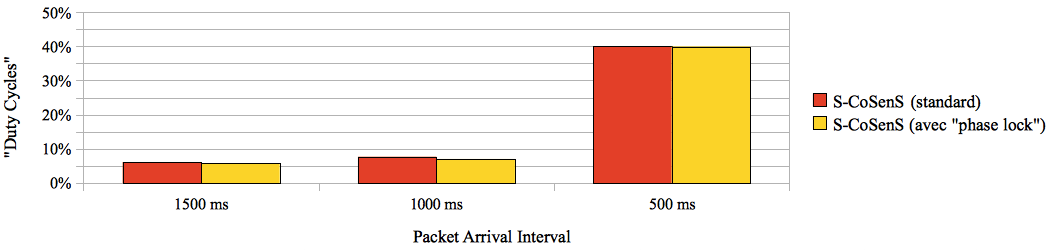
\includegraphics[width=14cm]{images/ch5-duty-cycles-pl-31ms.png}
\flcaption{Influence du mécanisme de \lang{``phase lock''} sur l'activité
radio (\lang{duty cycle}) induite par S-CoSenS, avec des \lang{subframes}
de 31~ms.}
\label{FigDutyCyclesPhaseLock31ms}
\end{figure}


On remarque que seules les données pour les noeuds-feuilles sont présentées~:
cette optimisation ne s'applique pas au routeur, du fait de la conception
même du protocole S-CoSenS.

On voit également que les valeurs de <<~transmission efficace~>>,
<<~réception efficace~>>, et <<~interférences~>> sont identiques à celles
de la table \vref{TblDutyCyclesSCoSenS}. Notre optimisation tente en effet
de réduire le temps d'écoute <<~à vide~>> des noeuds-feuilles, lors de
l'attente de réception des \lang{``beacons''}. Seules les valeurs de la
ligne <<~activité radio~>> varient donc par rapport aux résultats
du protocole S-CoSenS standard.

Ces valeurs <<~d'activité radio~>> totale sont effectivement moins élevées
par rapport au protocole S-CoSenS standard, mais la baisse de ces valeurs
reste relativement limitée, tout spécialement lors des forts trafics réseau~:
à un intervalle d'émission des trames de 500~ms, la baisse de valeur
d'activité radio est à peine perceptible. Ceci est logique~: dans une telle
configuration, la majorité de l'activité radio a lieu lors de la période
d'écoute du routeur (WP), et les nombreuses collisions sont responsables
de l'activité radio intense nécessaire pour pouvoir réussir à faire passer
les trames (nombreux réessais).

Avec des débits plus modérés (une trame toute les 1000 et 1500~ms),
la baisse est plus sensible, et permet de se rapprocher des (et même dans
un cas descendre sous les) valeurs d'activité radio constatées pour les
noeuds-feuilles sous ContikiMAC. Néanmoins, la baisse de valeur d'activité
radio due à la modification de S-CoSenS reste limitée~: étant donné que
S-CoSenS ne nécessite pas de répéter continuellement l'envoi des trames
jusqu'à réception par le destinataire (contrairement à ContikiMAC), on peut
être déçu de ne pas repasser systématiquement et surtout significativement
sous les valeurs d'activité radio de ContikiMAC.

\medskip

Nous avons retenté nos simulations, pour évaluer les \lang{``duty cycles''}
de ContikiMAC et S-CoSenS avec optimisation de type \lang{``phase-lock''},
cette fois avec une durée de cycle plus longue. Les résultats sont
visibles respectivement dans les tables
\vref{TblDutyCyclesContikiMACCycleLong} et
\vref{TblDutyCyclesSCoSenSPhaseLockCycleLong}, dans lesquelles nous
n'avons reporté que les valeurs des lignes <<~Activité radio~>> des
noeuds-feuilles, étant donné que nous avons vu que les autres valeurs
n'étaient pas affectées par cette optimisation. (Rappelons que dans cette
configuration~--- cycles de 125~ms~---, S-CoSenS obtient des résultats
largement meilleurs en termes de qualité de service que ContikiMAC,
comme vu dans les sections \vrefrange{SubsecTRP}{SubsecDelaiTransm}.)

Ces résultats sont également illustrés par la figure
\vref{FigDutyCyclesPhaseLock125ms}.


%%% duty cycles pour ContikiMAC avec cycle long
\begin{table}[htbp]
\centering
\begin{tabular}{|l|r|r|r|}
\hline
\multicolumn{4}{|c|}{ContikiMAC~: \lang{Channel Check Interval} = 8~Hz}\\
\hline
 INTERVALLE D'\'EMISSION DES TRAMES & 1500 ms & 1000 ms & 500 ms \\
\hline
 NOEUDS-FEUILLES (moyenne) & \multicolumn{3}{|c|}{ }\\
\hline
Activité radio             &  3,38\% &  3,87\% &  4,79\% \\
\hline
\end{tabular}
\flcaption{Statistiques de \lang{duty cycle} pour ContikiMAC avec un
cycle long~: CCI de 8~Hz (valeur par défaut), soit un cycle de 125~ms.}
\label{TblDutyCyclesContikiMACCycleLong}
\end{table}


%% duty-cycles pour S-CoSenS avec cycle long
\begin{table}[hbtp]
\centering
\begin{tabular}{|l|r|r|r|}
\hline
\multicolumn{4}{|c|}{S-CoSenS~:
                     Durée d'un cycle (\lang{subframe}) = 125~ms}\\
\hline
 INTERVALLE D'\'EMISSION DES TRAMES & 1500 ms & 1000 ms & 500 ms \\
\hline
 NOEUDS-FEUILLES (moyenne) & \multicolumn{3}{|c|}{ }\\
\hline
Activité radio (protocole standard) &  9,02\% & 11,45\% & 27,37\% \\
Activité radio (avec \lang{``phase lock''})
                                    &  4,61\% &  5,82\% & 17,26\% \\
\hline
\end{tabular}
\flcaption{Statistiques de \lang{duty cycle} pour S-CoSenS au niveau
des noeuds-feuilles, avec une \lang{subframe} longue de 125~ms.}
\label{TblDutyCyclesSCoSenSPhaseLockCycleLong}
\end{table}


%% figure de comparaison des duty-cycles avec cycles longs
\begin{figure}[htbp]
\centering
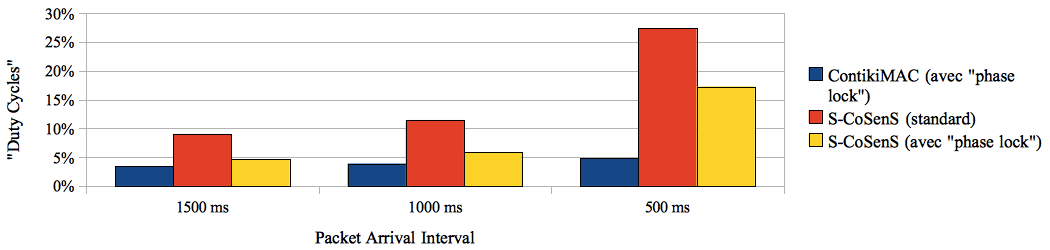
\includegraphics[width=14cm]{images/ch5-duty-cycles-pl-125ms.png}
\flcaption{Influence du mécanisme de \lang{``phase lock''} sur l'activité
radio (\lang{duty cycle}) induite par S-CoSenS et ContikiMAC, avec
respectivement des \lang{subframes} de 125~ms et des CCI de 8~Hz.}
\label{FigDutyCyclesPhaseLock125ms}
\end{figure}


On voit ici qu'avec une durée de \lang{subframe} plus longue,
le taux d'activité radio sous S-CoSenS baisse de façon significative avec
le mécanisme de \lang{``phase-lock''}~: de l'ordre d'un tiers d'activité
en moins avec un trafic réseau élevé (intervalle d'émission des trames de
500~ms), et une réduction de moitié de l'activité radio pour les charges
réseau plus modérées (intervalle d'émission des trames égal ou supérieur
à une seconde). Ce résultat est très intéressant, compte-tenu de la
supériorité de S-CoSenS du point de vue de la QdS dans cette situation.

Par contre, on voit que là encore, même si la baisse du pourcentage
d'activité radio devient importante au niveau de S-CoSenS avec une durée
de \lang{subframe} plus longue, ContikiMAC garde un \lang{duty cycle}
nettement inférieur.

\bigskip

Nous expliquons la relative importance des valeurs de \lang{duty cycle} 
de S-CoSenS~--- par rapport à ContikiMAC~--- de la façon suivante~:
outre la \lang{``subframe''} de longueur connue à l'avance, S-CoSenS
intègre dans son cycle une phase de transmission dont la durée reste
inconnue jusqu'à sa fin, puisque cette durée dépend du nombre de trames
à transmettre et du temps nécessaire pour les transmettre (éventuelles
interférences et collisions). Ainsi, S-CoSenS a toujours des cycles de
durée variable, tandis que l'intervalle entre deux cycles~--- c.-à-d.
deux CCA consécutifs~--- est toujours constant pour ContikiMAC quelles
que soient les circonstances (revoir les sections \vref{ParContikiMAC} et
\vref{ParSCoSenS} pour le détail du fonctionnement de ces deux protocoles).

Il est clair qu'un mécanisme du type \lang{``phase-lock''}, qui retient
la durée de cycle d'un récepteur pour optimiser les temps d'activation
des émetteurs, fonctionnera bien mieux avec un protocole à durée de cycle
constante comme ContikiMAC qu'avec un protocole auto-adaptatif comme
S-CoSenS ayant des cycles de durée variable et difficilement prévisible.

\bigskip

Ainsi, nous pouvons penser que~:

\begin{itemize}

\item \emph{l'implantation d'un mécanisme de type \lang{``phase-lock''}
se justifie pour S-CoSenS lorsqu'il est configuré avec une durée de
cycle (i.e.~: \lang{``subframe''}) suffisamment longue, là où les baisses
d'activité radio sont significatives, et de surcroît l'avantage de S-CoSenS
en termes de qualité de service est flagrant} (revoir sections
\vrefrange{SubsecTRP}{SubsecDelaiTransm})~;

\item par contre, \emph{la complexité supplémentaire introduite par l'ajout
d'un mécanisme de type \lang{``phase-lock''} au sein d'un protocole à durée
de cycle variable comme S-CoSenS ne se justifie guère lors de cycles
de fonctionnement (\lang{``subframes''}) courts, surtout en présence de
trafics réseau intenses, au vu des résultats forcément limités qu'apportera
dans de telles conditions un tel mécanisme} (à cause notamment de la grande
variabilité des durées de cycles)~;

\item \emph{un mécanisme de type \lang{``phase-lock''} devrait être assez
avantageux dans tous les cas pour envisager son implantation dans les
protocoles MAC~/ RDC à durée de cycle fixe et~/ ou connue à l'avance},
à condition bien sûr que la conception du protocole le permette.

\end{itemize}

%%%%%%%%%%%%%%%%%%%%%%%%%%%%%%%%%%%%%%%%%%%%%%%%%%%%%%%%%%%%%%%%%%%%%%%%%%%%%

\section[Discussion~: évaluation et comparaison de protocoles MAC~/ RDC,
         contributions et conclusion]
        {Discussion~: évaluation et comparaison de protocoles MAC~/ RDC,
         contributions et conclusion%
         \sectionmark{Discussion~: protocoles MAC~/ RDC,
                      contributions et conclusions}}
\sectionmark{Discussion~: protocoles MAC~/ RDC, contributions et conclusions}
\label{SecDiscussContribConcluProtocolesMAC}

Nos travaux ont permis de tester et comparer deux implantations complètes
et fonctionnelles de deux protocoles MAC~/ RDC, ContikiMAC et S-CoSenS.
Ces travaux ont consisté en des scénarios simulant de lourdes charges
réseau, dans le but d'observer la capacité de ces protocoles à monter
en charge, puis à les pousser dans leurs limites ultimes de fonctionnement~---
tout en sachant qu'approcher la limite théorique de 250~Kbit/s de bande
passante pour le médium radio physique défini par le standard IEEE
802.15.4 est impossible, à cause des délais imposés par le standard
lui-même (SIFS, LIFS), des limites matérielles des émetteurs~/ récepteurs
radio, et des délais occasionnés par les différentes couches des piles
réseau (et notamment les couches MAC et RDC).

Nous avons, durant l'implantation de S-CoSenS sur RIOT OS, surmonté
de nombreux problèmes dont nous avons discuté dans le présent chapitre.

Ce faisant, nous avons \emph{fourni les contributions suivantes}~:

\begin{itemize}

\item Nous avons d'abord \emph{prouvé que Cooja (le simulateur de WSN du
projet Contiki) n'était nullement limité à cette plate-forme logicielle}.
Nous l'avons employé avec succès pour tester des applications conçues sous
RIOT OS, et \emph{nous sommes convaincus que celui-ci peut servir à la
simulation de WSN fonctionnant avec n'importe quelle plate-forme logicielle,
ou même sans (programmation \lang{``bare metal''})}, et ce grâce au recours
à des émulateurs pour la gestion des \lang{motes} virtuelles.

\item Nous avons montré que des \emph{fonctionnalités temps-réel sont
nécessaires} pour implanter des protocoles MAC~/ RDC novateurs et
efficaces. Plus précisément~: une résolution temporelle à fine
granularité (nécessairement inférieure à la milliseconde, une résolution
de l'ordre de 30~microsecondes étant tout à fait satisfaisante), et la
disponibilité de plusieurs \lang{timers} offrant cette fine granularité
temporelle~--- l'usage d'au moins un \lang{timer} matériel étant en général
nécessaire pour atteindre un tel but.

\item Nous avons montré que \emph{notre implantation du protocole
S-CoSenS présente un avantage en termes de QdS} (TRP et délais de
transmissions) \emph{particulièrement en présence d'un trafic réseau
intense}, tandis que ContikiMAC (dans son implantation standard
sous Contiki) est largement supérieur en terme de \lang{duty cycles}.

\item Nous avons envisagé des \emph{contre-mesures pour gérer les erreurs
liées à des problèmes de corruption mémoire} (comme l'écrasement par
la pile système d'autres données, à cause de l'espace mémoire
très limité sur les \lang{motes} de base).
Notamment~--- sur les architectures matérielles dépourvues de circuit
MPU dédié~--- la nécessité de surveiller régulièrement la pile système,
\emph{de préférence par l'insertion automatique de code de vérification,
durant le processus de compilation,} à des endroits stratégiques du chemin
de code (appels de sous-programmes, interruptions, etc.).

\item Nous avons \emph{évalué l'influence des optimisations des
implantations sur les performances}, notamment dans la gestion du bus SPI,
selon le traitement des transmissions d'une façon sûre ou au contraire
optimisée~: le choix de l'une ou l'autre des solutions impacte la vitesse
de chargement des trames dans l'émetteur~/ récepteur radio d'un facteur
2 à 3, cette accélération se faisant au détriment de la fiabilité.
Notons toutefois que cette différence ne semble pas avoir changé
significativement les résultats globaux de nos comparaisons.

\item Nous avons enfin \emph{proposé des idées d'améliorations
algorithmiques au protocole S-CoSenS} (liées à l'optimisation des periodes
de réveil de l'émetteur~/ récepteur radio, à l'estimation du trafic réseau
et à l'optimisation du SNR), \emph{et à notre sens facilement généralisables
à de nombreux protocoles MAC~/ RDC}, si ce n'est~--- pour la dernière de
ces trois améliorations~--- à toutes les couches basses des piles réseau
des plates-formes logicielles destinées aux WSN.

\end{itemize}

En conclusion, nous avons constaté qu'il est essentiel pour un protocole
MAC~/ RDC d'être capable de traiter efficacement une lourde charge réseau
(ou des pointes de trafic), tout en gardant un \lang{duty cycle} minimal
durant les périodes de faible trafic.

Ces deux objectifs contradictoires doivent faire l'objet d'un compromis,
dont dépend le choix d'un protocole MAC~/ RDC et éventuellement la
configuration de celui-ci.

Notre conviction est toutefois qu'un WSN est \emph{d'abord} déployé pour
communiquer des informations, et doit donc \emph{en priorité} transmettre
le trafic réseau quand celui-ci apparaît. L'économie d'énergie est le
\emph{deuxième} objectif principal, pour allonger la durée de fonctionnement
et~/ ou de vie des noeuds du WSN, mais ne doit jamais~--- selon nous~---
se faire au détriment de la qualité de service <<~fonctionnelle~>>.

\emph{C'est pourquoi nous pensons qu'un protocole MAC~/ RDC idéal
est un protocole dont le \lang{``duty cycle''} doit varier dynamiquement
en fonction du trafic, certes pour permettre d'optimiser la consommation
d'énergie, mais jamais au prix de la perte de données à transmettre
(sauf bien sûr dans les cas de saturation du médium radio).}

\bigskip

Pour finir, rappelons que lors de nos tests concernant l'influence
de l'optimisation des implantations sur les performances (section
\vref{SubsecOptim}), nous avions observé des incohérences dans les
valeurs obtenues entre simulation et exécution sur matériel réel, tout
particulièrement en ce qui concerne la plate-forme matérielle Zolertia Z1.
Comme nous l'avions alors dit, nous allons maintenant étudier ce phénomène
en détail dans la section \ref{SecLimInexactSimu} du chapitre suivant.


%%%%%%%%%%%%%%%%%%%%%%%%%%%%%%%%%%%%%%%%%%%%%%%%%%%%%%%%%%%%%%%%%%%%%%%%%%%%%
%%%                 FIN DU CHAPITRE "PROTOCOLES MAC/RDC"                  %%%
%%%%%%%%%%%%%%%%%%%%%%%%%%%%%%%%%%%%%%%%%%%%%%%%%%%%%%%%%%%%%%%%%%%%%%%%%%%%%

